\documentclass[article]{jss}
\usepackage[utf8]{inputenc}
\usepackage[]{amsmath}
\usepackage{amssymb}
\usepackage{enumerate}
\pdfinclusioncopyfonts=1

\DeclareMathOperator*{\argmin}{arg\,min}
\DeclareMathOperator*{\argmax}{arg\,max}

%%%%%%%%%%%%%%%%%%%%%%%%%%%%%%
%% declarations for jss.cls %%%%%%%%%%%%%%%%%%%%%%%%%%%%%%%%%%%%%%%%%%
%%%%%%%%%%%%%%%%%%%%%%%%%%%%%%

%% almost as usual
\author{Daniel Kaschek\\University of Freiburg \And
	Marcus Rosenblatt\\University of Freiburg \AND
	Wolfgang Mader\\University of Freiburg \And
	Mirjam Fehling-Kaschek\\University of Freiburg \And
	Jens Timmer\\University of Freiburg}

\title{Dynamic Modeling, Parameter Estimation and Uncertainty Analysis in \proglang{R}}

%% for pretty printing and a nice hypersummary also set:
\Plainauthor{Daniel Kaschek, Marcus Rosenblatt, Wolfgang Mader, Mirjam Fehling-Kaschek} %% comma-separated
\Plaintitle{Dynamic Modeling and Parameter Estimation in R} %% without formatting
\Shorttitle{Dynamic Modeling} %% a short title (if necessary)

%% an abstract and keywords
\Abstract{
In a wide variety of research fields, dynamic modeling is employed as an instrument to learn and understand complex systems. The differential equations involved in this process are mostly non-linear and depend on many parameters which decide upon the characteristics of the emergent system. The inverse problem, i.e.~the inference or estimation of parameter values from observed data, is interesting from two points of view. First, the existence point of view, dealing with the question whether the system is able to  produce the observed dynamics for any parameter values. Second, the identifiability point of view, investigating invariance under change of parameter values and quantifying parameter uncertainty.

In this paper, we present the \proglang{R} package \pkg{dMod} providing a framework for dealing with the inverse problem in dynamic systems. The particularity of the \pkg{dMod} approach is to provide and propagate accurate derivatives computed from symbolic expressions wherever possible. This derivative information highly supports the convergence of optimization routines and enhances the numerical stability required by sofisticated uncertainty analysis methods. Computational efficiency is guaranteed by automatic generation and integration of \proglang{C} code. The framework is object oriented (S3) and provides a variety of functions to set up dynamic models, observation functions and parameter transformations for multi-conditional parameter estimation. 

The key elements of the framework and the methodology implemented in \pkg{dMod} are highlighted by an application on a three-compartment transporter model within this paper.



%First, the question is if there exist any parameters such that the dynamic system is able to produce the observed dynamics and second, how well are the parameters determined by the data.


}
\Keywords{Dynamic models, parameter estimation, code generation, maximum likelihood}
\Plainkeywords{Dynamic models, parameter estimation, code generation, maximum likelihood} %% without formatting
%% at least one keyword must be supplied

%% publication information
%% NOTE: Typically, this can be left commented and will be filled out by the technical editor
%% \Volume{50}
%% \Issue{9}
%% \Month{June}
%% \Year{2012}
%% \Submitdate{2012-06-04}
%% \Acceptdate{2012-06-04}

%% The address of (at least) one author should be given
%% in the following format:
\Address{
  Daniel Kaschek\\
  Institute of Physics, University of Freiburg\\
  Hermann-Herder-Str.~3\\
  79104 Freiburg, Germany\\
  E-mail: \email{daniel.kaschek@physik.uni-freiburg.de}
  %URL: \url{http://eeecon.uibk.ac.at/~zeileis/}
}
%% It is also possible to add a telephone and fax number
%% before the e-mail in the following format:
%% Telephone: +43/512/507-7103
%% Fax: +43/512/507-2851

%% for those who use Sweave please include the following line (with % symbols):
%% need no \usepackage{Sweave.sty}

%% end of declarations %%%%%%%%%%%%%%%%%%%%%%%%%%%%%%%%%%%%%%%%%%%%%%%


\begin{document}

%% include your article here, just as usual
%% Note that you should use the \pkg{}, \proglang{} and \code{} commands.
\section{Introduction}
Dynamic models are found in several research fields, such as physics, biology or finance. In all these fields, models are used to construct a link between theoretical concepts and empirical evidence. In a dynamic model, the single terms correspond to mechanisms or processes which are combined to a whole, giving rise to a complex system. If the single terms are associated to parameters, parameter estimation can identify those processes which are crucial to explain the observation. In that sense, parameter estimation can be employed as an instrument to \textit{understand} complex systems. Once, the link between observation and model is established, questions about the identifiability of parameters arise. The parameter space needs to be explored to analyze whether the estimate is unique and to determine confidence bounds.

Although the problem of parameter estimation in non-linear dynamic systems is highly relevant and at the heart of statistical computing, to this day there are not more than four \proglang{R} packages published on the topic on the Comprehensive \proglang{R} Archive Network (CRAN), namely \pkg{FME} \citep{FME}, \pkg{nlmeODE} \citep{nlmeODE}, \pkg{mkin} \citep{mkin} and \pkg{scaRabee} \citep{scaRabee}. All packages have in common that they are built upon the \pkg{deSolve} package \citep{deSolve}.
The packages \pkg{mkin} and \pkg{FME} support ODEs defined by compiled code where \pkg{mkin} provides tools to autogenerate the \proglang{C} code and compile it using the \pkg{inline} package. For model fitting and uncertainty analysis, \pkg{mkin} fully resorts to the functionality of \pkg{FME}.
Concerning model fitting, \pkg{FME} and \pkg{nlmeODE} (with \pkg{nlme} in the background) use deterministic derivative-based optimizers by default, i.e.~either Levenberg-Marquardt or Newton methods provided by \code{nls.lm()}, \code{optim()} or \code{nlmimb()}. Although all these optimizers support gradient or Hessian information as input, only the \pkg{nlmeODE} package provides an option to augment the ODE by its sensitivity equations to generate derivates for the residuals. By default, sensitivities are computed by finite differences. Last but not least, the \pkg{scaRabee} package uses the Nelder-Mead optimization algorithm which is derivative-free but needs in general more iterations until convergence.
In all packages, uncertainty analysis is by default based on the variance-covariance matrix, i.e.~on the inverse Hessian matrix of the least squares function. For non-linear models, this method provides a good approximation only if parameters are identifiable and the data is highly informative. If these conditions are not met, more sophisticated methods like e.g.~Markov chain Monte Carlo (MCMC) sampling, implemented in \pkg{FME}, are required.
The strength of \pkg{scaRabee} and especially \pkg{nlmeODE} is multi-conditional fitting. This means that the same model with the same parameters but different forcings to reflect experimental conditions is fitted simultaneously to the condition-specific data sets. In the context of mixed-effects modeling as provided by \pkg{nlmeODE}, parameters can be grouped in fixed effects (same parameters over all conditions) and random effects (parameters are different between conditions).  

In this paper we present \pkg{dMod}, an \proglang{R} package on dynamic modeling and parameter estimation. The aim and core functionality of \pkg{dMod} is
\begin{enumerate}[(i)]
	\item facilitated set-up of dynamic models with automated \proglang{C} code generation for fast simulation of model predictions and model sensitivities,
	\item flexible set-up of general parameter transformations (explicit or implicit) and observation functions, allowing for the implementation of multiple experimental conditions similar to mixed-effects modeling,
	\item parameter estimation based on trust-region optimization of the negative log-likelihood, making use of the sensitivity equations of the dynamic system and of symbolic derivatives of the observation- and parameter transformation functions,
	\item identifiability and uncertainty analysis based on the profile-likelihood method to determine confidence intervals for parameters and predictions.
\end{enumerate}

The core functionality is extended by two symbolic methods implemented in \proglang{Python} and interfaced via the \pkg{rPython} package: identifiability and observability analysis based on Lie-group symmetries \citep{merkt2015higher} and steady-state constraints for parameter estimation \citep{rosenblatt2016customized}.

The strict implementation of capabilities to generate and propagate derivatives on a compiled-code level distinguishes \pkg{dMod} from other modeling frameworks as discussed above. Most of the standard optimization routines implemented in \proglang{R} need derivative information. However, the computation of derivatives in the context of ODE models holds some pitfalls. The accuracy of sensitivities obtained from finite differences can be insufficient because the step control of the integrator presents an additional source of numeric inaccuracy. Even for numeric methods circumventing this problem, e.g.~complex-step derivatives \citep{squire1998using}, the use of sensitivity equations is still beneficial judging from the accuracy vs.~computational cost ratio. See \citep{raue2013lessons} for a comparison of methods.

Another distinguishing feature of \pkg{dMod} is the handling of non-identifiability of parameters, a phenomenon occurring frequently in the context of parameter estimation in dynamic systems.
 In some cases, non-identifiability has structural reasons. The differential equations bear certain symmetries and these can or cannot be broken by observation functions. A functional relationship between parameters that leaves the observation invariant is the consequence of the latter. In other cases, the data allows to determine a unique optimum but other solutions, although worse, cannot be statistically rejected. The \pkg{dMod} package deals with parameter identifiability and parameter uncertainty by the profile-likelihood method \citep{murphy2000profile, kreutz2013profile}. The method has proven especially useful in the case of non-identifiable parameters where results obtained from both, the quadratic approximation by the variance-covariance matrix and MCMC sampling can be misleading \citep{raue2013joining}. Besides parameter uncertainties, the profile likelihood method allows to estimate prediction uncertainty, it supports the planning of new informative experiments or suggest possible model reductions.

The key methods implemented in \pkg{dMod} are illustrated in great detail on a dynamic model of bile acid flow. The example is a show-case of how modeling \textit{is} a dynamic process, using the analysis tools implemented in \pkg{dMod} to predict, plan new experiments, combine data from different experiments and include non-linear parameter constraints to improve parameter identifiability. Thereby, we show that \pkg{dMod} is a full-grown, flexible modeling environment, fast, thanks to compiled code, reliable, thanks to symbolic derivatives, and accurate, thanks to advanced statistical methods. 

The paper is organized as follows: Section~\ref{sec:theory} introduces the mathematical set-up of dynamic modeling, symmetries in dynamic systems, parameter estimation by the maximum-likelihood method and the profile likelihood. Section~\ref{sec:implementation} discusses the implementation and design principles behind the \pkg{dMod} software. The functionality of \pkg{dMod} is presented in Section~\ref{sec:example} on the example of bile acid flow in a three-compartment model and finally, Section~\ref{sec:extensions} discusses the two \proglang{Python} extensions coming with \pkg{dMod}.


% Rechenzeit erwähnen



\section{Theoretical background}
\label{sec:theory}

\subsection{Dynamic models and model sensitivities}
Dynamic models describe systems with states $x$, usually quantifying the involved species, interacting and evolving over time. %  as e.g. given by chemical reaction networks. 
The time evolution of the states is expressed via a set of ODEs, $\dot x = f(x)$. Although constituting quite a special class of dynamic systems, chemical reaction networks formulated by the law of mass action allow for surprisingly general applications. Typical ODE examples derived from the law of mass action are:
\begin{itemize}
	\item $\dot x_A = k_p$ constant production of $x_A$ ($\emptyset \rightarrow A$)
	\item $\dot x_C = k_c \cdot x_A \cdot x_B = - \dot x_A = - \dot x_B$ complex formation ($A+B \rightarrow C$)
	\item $\dot x_C = - k_d \cdot x_C$ constant degradation of $x_C$ ($C \rightarrow \emptyset$)
\end{itemize}
each generally written as 
\begin{align}
	\dot x = \underbrace{k_0 \left(\prod x_i^{\nu_i}\right)}_{v_0(x, k_0)} (\nu' - \nu) \quad\leftrightarrow\quad (\nu_1 X_1 + \dots + \nu_n X_n \longrightarrow \nu'_1 X_1 + \dots + \nu'_n X_n)
	\label{eq:ma}
\end{align}
where $X_1, \dots, X_n$ are the $n$ species involved, $\nu$ and $\nu'$ encode the stoichiometry of the reaction and $k_0$ is the reaction rate. When several reactions are involved, eq.~\eqref{eq:ma} generalizes to 
\begin{align}
	\dot x = S\cdot v(x, k)
	\label{eq:Sv}
\end{align}
%$\dot x_l = \sum_{j = 1\dots m}  k_{j} \prod_{i = 1\dots n} \nu_{i,j} x_i^{\nu_{i,j}}$ for a system of $n$ states and $m$ reactions with rate constants $p = \{ k_j, j = 1\dots m\}$ and stoichiometric constants $\nu_{i,j} \in \mathbb{Z}$. 
%An even more general expression of the system is given by $\dot x = S v(x,p)$ 
with the stoichiometry matrix $S$
%containing the stoichiometric constants $\nu_{i,j}$ 
obtained from the collection of vectors $\nu' - \nu$ for reactions $1, \dots, r$,
and the flux vector $v(x,k)\in\mathbb R^{r}$.
Eq.~\eqref{eq:Sv} also holds for general ODEs that do not follow from mass action kinetics. Moreover the system may be explicitly time-dependent and may contain forcings $u(t)$ which e.g.~describe the external stimulation of the system. A general form of the dynamic model is therefore given by
\begin{align} 
	\dot x = f(x,k,u,t) = S \cdot v(x,k,u,t), \quad\quad \textrm{with }  x(t = 0) = x_0.
\end{align}
The solution $x(t,\theta)$ for a given parameter vector $\theta = (k, x_0)$ is called model prediction. %The parameters $\theta$ contain the rate constants, initial values $x_0$ and additional parameters included in the forcings. 
It is generally assumed that the stoichiometry matrix $S$ of the system is known.
Besides the model predition itself, also the sensitivity of the prediction to changes in the parameter values is of interest. 
The sensitivities $s_i = \frac{\partial x}{\partial \theta_i}$ satisfy the \textit{sensitivity equations}
\begin{align}
	\dot s_i  = \frac{\partial f}{\partial x} s_i + \frac{\partial f}{\partial \theta_i}, \qquad \textrm{with }s_i(t = 0) = \frac{\partial x_0}{\partial \theta_i},
\end{align}
a system of ordinary differential equations that in general depend on the states $x$ and, therefore, need to be solved jointly with the original ODE. 

Often the experimentally observed quantities $y$ do not directly correspond to the species $x$ described by the ODE, but are obtained via an observation function $g: \mathbb{R}^n \rightarrow \mathbb{R}^m$,  \begin{align}
	y = g(x, c)
\end{align}
with the observation parameters $c$. Examples for observation functions are scaling and offset transformations, $y = c_s \cdot x + c_o$, or the measurement of a superposition of species, $y_i = \sum_j c_j x_j$. The model prediction for the observed states is obtained by evaluating the observation function on the solution of the ODE. Following the chain rule of differentation also the sensitivities of the observed states $\frac{\partial y}{\partial \theta_i} = \frac{\partial g}{\partial x} \frac{\partial x}{\partial\theta_i}  + \frac{\partial g}{\partial \theta_i}$ are obtained. Here, the parameter vector $\theta$ has been augmented by the observation parameters, $\theta = (k, x_0, c)$.

The estimation of the parameters $\theta$ given the observation $y(t)$ is addressed in the next section.
%Next, the question how to estimate the parameters $\theta$ given the observation $y(t)$ is addressed.

% Eventuell of multi-condition prediction

% Statistical model um Überleitung zum nächsten Abschnitt zu machen

\subsection{Maximum-likelihood method}

Parameter estimation is a common task in statistics. It describes the process of inferring parameter values or parameter ranges of a statistical model based on observed data. Over decades, appropriate estimators have been developed for different problem classes. The principle of maximum likelihood allows to derive an estimator which is especially suited for applications where the distribution of the measurement noise is known. This knowledge about the structure of the noise constitutes additional information that makes the maximum-likelihood estimator (MLE) \textit{efficient}, i.e.~from all unbiased estimators the MLE has the lowest variance. Other properties of maximum-likelihood estimation are \textit{consistency}, i.e.~the true parameter is reached in the limit of infinite data-sample size, and \textit{asymptotic normality}, i.e.~in the limit of infinite data the MLE follows a multivariate normal distribution. See \citep{azzalini1996statistical} for an introduction to likelihood theory.

Maximum-likelihood estimation is based on the maximization of the likelihood function $L(\theta) = \phi(y^D|\theta)$. Here, $\phi$ is the joint probability density for a vector of observations $y$ evaluated at the point $y = y^D$, the vector of data points. The distribution $\phi$ depends parametrically on model parameters $\theta$. The maximum-likelihood estimator $\hat\theta$ is defined as
\begin{align*}
	\hat \theta := \argmax_{\theta} L(\theta),
\end{align*}
meaning that $\hat\theta$ is an extremum estimator. Depending on the model class and the probability distribution $\phi$, maximization of the likelihood can be a challenge beyond the scope of analytical methods. Numerical optimization methods help to solve the maximization problem in practical applications.

The easiest and one of the most frequent situations is when $\phi$ follows a normal distribution, $\phi\sim\mathcal N(\mu(\theta), \Sigma)$. When measurements are statistically independent, the variance-covariance matrix $\Sigma$ is diagonal and $\phi$ factorizes. The Likelihood function becomes
\begin{align}
	L(\theta) &= \prod_i \frac{1}{\sqrt{2\pi\sigma_i^2}} e^{-\frac{\mu_i(\theta)^2}{2\sigma_i^2}} 
	\label{eq:likelihood}
\end{align}
The connection between the statistical model and the observed data is given by $\mu_i(\theta) = y_i(\theta) - y_i^D$. Taking twice the negative logarithm, eq.~\eqref{eq:likelihood} turns into
\begin{align}
	l(\theta) = -2\log L(\theta) &= \sum_i \left[\left(\frac{y_i(\theta) - y_i^D}{\sigma_i}\right)^2 + \log(2\pi\sigma_i^2)\right],
	\label{eq:nll}
\end{align}
thus converting the maximization of $L(\theta)$ to a minimization of $l(\theta)$. 
Assuming that the data uncertainties $\sigma_i$ are known, eq.~\eqref{eq:nll} is the weighted least-squares function shifted by a constant. For unknown $\sigma_i$, eq.~\eqref{eq:nll} can be optimized with respect to $\theta$ and $\sigma$ jointly, yielding the MLE $\hat\theta^{\prime} = (\hat\theta, \hat\sigma)$.

\subsection{Non-linear optimization}

Numerical optimization is a diverse field with as many algorithms as there are optimization problems around. For our application, derivative-based methods and in particular the Newton method plays a major role.

Optimization by the Newton method attempts to iteratively find the root of the gradient $\nabla l (\theta)$ by the recursion
\begin{align}
	\theta^{(n+1)} = \theta^{(n)} - Hl(\theta)^{-1}\nabla l(\theta),
	\label{eq:newton}
\end{align}
where $Hl(\theta)$ denotes the Hessian, i.e.~the matrix of second derivatives of $l(\theta)$. The fact that for normally distributed noise the log-likelihood is a least squares function, has a big advantage: gradient and (approximate) Hessian can be computed from first-order derivatives,
\begin{align}
	\nabla l(\theta) = 2 r(\theta) J(\theta) \quad\quad Hl(\theta) \approx 2 J(\theta)^T J(\theta),
	\label{eq:derivatives}
\end{align}
with the weighted residual vector $r_i(\theta) = \frac{y_i(\theta) - y_i^D}{\sigma_i}$ and its first derivative, the Jacobian matrix 
\begin{align}
	J_{ij}(\theta) = \frac{\partial r_i}{\partial \theta_j}(\theta) = \frac{1}{\sigma_i} \frac{\partial y_i}{\partial \theta_j}(\theta). \label{eq:jacobian}
\end{align}
As indicated by eqs.~\eqref{eq:derivatives}-\eqref{eq:jacobian},  first model sensitivities $\frac{\partial y_i}{\partial\theta_j}$ are sufficient to compute gradient and Hessian in good approximation.

The Newton recursion, eq.~\eqref{eq:newton}, converges in one iteration if $l(\theta)$ is a quadratic form. However, $l(\theta)$ is only quadratic if the model $y(\theta)$ is linear in $\theta$ which is usually not the case for ODE models. On the other hand, each smooth function, no matter if quadratic or not, can be approximated by a quadratic function based on its Taylor series. Depending on the function's shape, the \textit{trust region}, i.e.~the region where $l(\theta)$ is well approximated, can become quite small. Accordingly, a Newton step pointing far beyond this region could be misleading and not helpful for optimization. This is the idea behind trust-region optimization \citep{wright1999numerical}. In each iteration, the trust-region radius is adjusted and the optimization problem restricted to the trust region is solved. For parameter estimation in ODE models this has the additional advantage that parameter changes are constricted and optimization steps into parameter regions where the ODE cannot be numerically solved any more  become less frequent. This make trust-region optimization the method of choice for ODEs.



% Hier auf Maximum-Likelihood vs. least-squares function eingehen.

\subsection{Uncertainty analysis}

Parameter estimates $\hat \theta$  are obtained by non-linear optimization of the log-likelihood function $l(\theta)$. Although being a function of the parameters,  the log-likelihood depends on the data, too. Consequently, "equivalent" random ralizations of the data would lead to different parameter estimates $\hat\theta$. Given $\hat\theta$ for one random realization of the data, the question is, if we can reject other parameters $\theta$ with a certain confidence level. This leads to the related question of parameter convidence intervals.

A useful tool to derive confidence intervals is the profile likelihood. Consider a parameter of interest, $\theta_i$, being one of the parameters in the vector $\theta$. Furthermore, let $g_x(\theta) = \theta_i - x = 0$ be a parameter constraint. Then the function 
\begin{align}
	\begin{aligned}
		{\rm pl}_i:\quad \mathbb R & \longrightarrow \mathbb R\\
		x & \longmapsto \min_{(\theta, \lambda)} \big[ l(\theta) + \lambda g_x(\theta) \big]
	\end{aligned}
	\label{eq:pl}
\end{align}
is called the profile likelihood of the $i^{\;\rm th}$ paramameter and the path $x \mapsto (\hat\theta_x, \hat\lambda_x)$ along the minimizing parameters is called the profile likelihood path. Hence, the profile likelihood ${\rm pl}_i$  returns the minimal log-likelihood under the constraint $\theta_i \stackrel{!}{=} x$. By construction, the inequality $D := {\rm pl}_i(x) - {\rm pl}_i(\hat \theta_i) \geq 0$ holds for all $x$, assuming equality for $x = \hat\theta_i$. Interpreting the model with free $\theta$ as the null model and that with $\theta_i$ fixed to $x$ as the alternative model, the value $D$ is twice the log of the likelihood-ratio between those. Hence, a likelihood-ratio test can be performed to accept or reject the alternative model at a given confidence level. To compute the corresponding threshold, we assume Wilks' theorem according to which the thresholds are the quantiles of the $\chi^2$ distribution with one degree of freedom. Consequently, the $1\sigma, 2\sigma, \dots, n\sigma$-confidence intervals of $\theta_i$ are those values of $x$ for which ${\rm pl}_i(x) \leq 1, 2, \dots, n$, respectively. 

The reason to formulate the profile likelihood by Lagrangian multipliers is that we can directly use eq.~\eqref{eq:pl} to derive the profile likelihood path $(\hat \theta_x, \hat\lambda_x)$ with respect to $x$:
\begin{align}
	\frac{\rm d}{{\rm d} x}
	\begin{pmatrix}
		\hat\theta_x \\ \hat\lambda_x
	\end{pmatrix} =
	\begin{pmatrix}
		Hl(\hat\theta_x) & \nabla g_x(\hat \theta_x)\\
		\nabla g_x(\hat\theta_x)^T & 0
	\end{pmatrix}^{-1}
	\begin{pmatrix}
		0 \\ 1
	\end{pmatrix}.
	\label{eq:path}
\end{align}
Eq.~\eqref{eq:path} forms the basis of what is implemented in \pkg{dMod} for computing the profile likelihood.





\section{Implementation and design principles}
\label{sec:implementation}

The guideline of \pkg{dMod} is to provide a class structure for models, predictions, observations and parameter transformations that allows a flexible combination of many experimental conditions in one objective function to fit models to data. This flexibility is achieved by two concepts: (1) concatenation of functions by a \code{"*"} operator and (2) stacking of functions representing different conditions by a \code{"+"} operator. The handling and propagation of derivatives as part of the classes happens in the background. Methods for the generic \code{print()}, \code{plot()} and \code{summary()} functions are implemented for most outputs.

\subsection{Model  formulation}

A system of ordinary differential equation $\dot x = f(x, p, u, t)$ can be represented by a \code{character} vector of symbolic expressions, the right-hand side of the ODE, involving symbols for the states $x$, the parameters $p$, the forcings $u$ and the keyword \code{time} for $t$. The class provided by \pkg{dMod} for such objects is the \code{eqnvec} class which checks whether the character can be parsed and thus, can be interpreted as an equation.

There are several ways to define the differential equations. An \code{eqnvec} of equations can be explicitly formulated, analogously to a \code{c()} command. Especially for chemical reactions it can be tedious to keep track of all gain and loss terms. Therefore, \pkg{dMod} provides the \code{eqnlist} class which encodes the ODE by a list of (1) state names, (2) rate expressions, (3) compartment volumes and (4) the stoichiometric matrix. Each reaction flux occurs only once and the gain and loss is represented by the coefficients in the stoichiometric matrix. \pkg{dMod} supports the read-in of a csv file with the stoichiometric matrix and rate expressions and provides a function \code{addReaction()} to construct an \code{eqnlist} object step-by-step or add further reactions to an already existing \code{eqnlist}. The conversion to the (differential) equations is done by \code{as.eqnvec()} which does all the bookkeeping of gain and loss terms and volume ratios due to compartment transitions.

The paradigm of \pkg{dMod} is to make use of derivatives wherever possible. It is one of the core functionalities of the \pkg{cOde} package upon which \pkg{dMod} is based to augment a system of ODEs by its sensitivity equations. If many parameters are involved and the system consists of many states, the number of equations quickly grows and solving the equations can be considerably accelerated if compiled code is used. \pkg{dMod} provides the \code{odemodel} class. An object of class \code{odemodel} is generated from an \code{eqnlist} or \code{eqnvec}. In the background \proglang{C} code for the ODE and the combined system of ODE and sensitivity equations is generated, written into the working directory and compiled. The \code{odemodel} object keeps track of the shared objects and is the basis of a prediction function $x(t, p)$ which is generated by the \code{Xs()} command.

\subsection{Prediction functions}

\pkg{dMod} seeks to stay close to the mathematical formulation, i.e.~\code{x <- Xs(myodemodel)} will indeed return an \proglang{R} function, an object of class \code{prdfn}, which expects arguments \code{times} and \code{pars} and turns them into a model prediction. However, not only the solution $x(t)$ is returned, the sensitivities $\frac{\partial x}{\partial p}(t)$ are returned, too.

Besides parameters, the prediction might also depend on forcings $u(t)$ and sudden events, e.g.~setting states to 0 at a predefined point in time. Since forcings and events are by default not variable, they are defined for a prediction function the moment it is generated, \code{x <- Xs(odemodel, forcings = myforcings, events = myevents)}. The definitions of both, forcings and events, are compatible with the way they are defined in \pkg{deSolve}.

\subsection{Observation functions}

% Concatenation in Einleitungssatz erwähnen.

An observation function is a function $g(x, p_{\rm obs}, t)$ that evaluates the solution $x(t)$ together with additional (observation) parameters $p_{\rm obs}$. The function can explicitly depend on time~$t$. Similar to the ODE case, an observation function can be expressed as a character vector with names corresponding to the names of the observables and equations involving symbols for the states, parameters and the keyword \code{time}. An observation function is defined as an \code{eqnvec} and turned into an \proglang{R} function via \code{Y()}.

It is one of the fundamental concepts of \pkg{dMod} to allow concatenation of functions via the \code{"*"} operator. The mathematical formulation $y = g\circ x$, i.e.~$y(t, p) = (g\circ x)(t, p):= g(x(t, p), p, t)$ becomes \code{y = g*x} in \proglang{R}. To obtain derivatives $\frac{\partial y}{\partial p}$, the chain rule is applied, yielding $\frac{\partial y}{\partial p} = \frac{\partial g}{\partial x}\frac{\partial x}{\partial p} + \frac{\partial g}{\partial p}$. This means that \code{Y()} needs to be informed which symbols are states and parameters to generate the corresponding expressions $\frac{\partial g}{\partial x}$ and $\frac{\partial g}{\partial p}$. The observation function \code{g} takes care of computing theses derivatives from the symbolic expressions and doing the matrix multiplication with the sensitivities $\frac{\partial x}{\partial p}$ from the prediction function. Evaluation of symbolic expressions can become inefficient in \proglang{R}. Therefore, the observation function is usually translated into a \proglang{C} code and compiled.

When observation- and prediction functions are concatenated, the result is a prediction function, e.g.~\code{y = g*x} is the \proglang{R} function computing values $y(t)$ from the arguments \code{times} and \code{pars} via evaluation of the ODE and subsequent evaluation of the observation function. Two observation functions can be concatenated, too, yielding an observation function.

\subsection{Parameter transformations}

Parameter transformations are the key element of \pkg{dMod} to formulate different kinds of constraints and allow the combination of several experimental/modeling conditions in one parameter vector.

In principle, a parameter transformation $p = \Phi(\theta)$ is a (differentiable) function connecting \textbf{inner} parameters $p$ with \textbf{outer} parameters $\theta$. The rationale behind the distinction of inner and outer parameters is that the vector $p$ usually desribes those parameters defined in the model equations. The outer parameters $\theta$ refer to a convenient parameterization by which the model parameters are computed. Examples are a log-transform of the inner parameters, $\theta = \log(p) \Leftrightarrow p = \Phi(\theta) = e^{\theta}$, or parameter constraints like $(p_1, p_2) = (\theta_1, \theta_1 + \theta_2)$.

An \proglang{R} function of class \code{parfn} is produced by the \code{P()} command. Transformations can either be formulated explicitly or implicitly. In the explicit case, the function $p = \Phi(\theta)$ corresponds to an \code{eqnvec} whose names are the names of the inner parameters and entries are equations with symbols for the outer parameters. An implicit transformation has the form $f\big(p = \Phi(\theta), \theta\big) = 0$. In this case, $f$ is expressed by an \code{eqnvec} with equations containing symbols for $p$ and $\theta$ and the names of the \code{eqnvec} are the symbols for $p$.

Similar to prediction- and observation functions, parameter functions not only return parameter values but the Jacobian of the transformation, too. Exploiting the chain rule, the derivatives are propagated, allowing to define \code{y = g*x*p} which is a function returning $y(t, \theta)$ and $\frac{\partial y}{\partial \theta}(t)$, i.e.~\code{g*x*p} is a prediction function.

Let \code{g}, \code{x}, \code{p1} and \code{p2} be an observation-, a prediction- and two parameter transformation functions. Then \code{p1*p2} is a parameter transformation function, \code{x*p1} is a prediction function and \code{g*p1} is an observation function.
 
\subsection{Multi-conditional prediction}

A set of parameter values, forcings and events reflects a certain condition in which we find a dynamic system. By manipulation of the system, single parameters, forcings or events can be changed. It is a typical approach to systems inference to systematically perturb small parts of a dynamic system to reveal information about the underlying process. 

The aim of \pkg{dMod} is to allow for "simultaneous" predictions under several conditions and compare these predictions to the corresponding experimental data sets to estimate model parameters.
Different experimental conditions can be expressed by that fact that some parameters are different between conditions whereas others are common to all conditions. This situation occurs e.g.~if perturbation experiments are performed, affecting only few parts of a system.
%The full information contained in several perturbation experiments is only used if the multi-conditional model prediction is set up in a way that all model parameters not being changed from condition to condition correspond to exactly one parameter. On the other hand, parameters which are systematically perturbed correspond to different parameters.
Mathematically speaking, we want to construct a parameter transformation
\begin{equation}
	\begin{aligned}
		\Phi:\quad \mathbb R^p & \longrightarrow  \bigoplus_{i = 1}^n \mathbb R^q \\
		\theta & \longmapsto  \left(\Phi_1(\theta), \dots, \Phi_n(\theta)\right)
	\end{aligned}
	\label{eq:partrafo}
\end{equation}
where $i = 1, \dots, n$ corresponds to the different conditions. If all parameters are shared throughout all conditions, then $p = q$. If, however, all parameters are distinct, then $p = n\cdot q$. Perturbation experiments correspond to a situation where $p\gtrsim q$.

The \pkg{dMod} package allows to define transformations $\Phi$, see eq.~\eqref{eq:partrafo}, by the \code{"+"} operator: 
\begin{equation*}
\verb!p <- P(eqnvec1, condition = "one") + P(eqnvec2, condition = "two")!. 
\end{equation*}
All symbols from \code{eqnvec1} and \code{eqnvec2} are collected and their union constitutes the symbols of $\theta$. The evaluation \code{p(theta)} returns a list of length $n$ (in the example $n = 2$) with inner parameters. The \code{"+"} operator can be applied consecutively to add condition by condition.

Prediction- and observation functions are generalized to multiple conditions by the \code{"+"} operator, too. Mathematically speaking, they become
\begin{align*}
	\begin{aligned}
		x: &  & \mathbb R \times \bigoplus_{i = 1}^n \mathbb R^q & \longrightarrow  \bigoplus_{i = 1}^n \mathbb R^m \\
		 & & (t, p_1, \dots, p_n) & \longmapsto (x_1(t, p_1), \dots, x_n(t, p_n)) \\
		g: &  & \bigoplus_{i = 1}^n \mathbb R^m \times \bigoplus_{i = 1}^n \mathbb R^q\times \mathbb R& \longrightarrow  \bigoplus_{i = 1}^n \mathbb R^s \\
		& & (x_1(t), \dots, x_n(t), p_1, \dots, p_n, t) & \longmapsto (g_1(x_1(t), p_1, t), \dots, g_n(x_n(t, p_n), p_n, t)).
	\end{aligned}
	\label{}
\end{align*}
In words, if prediction- or observation functions are defined for different conditions then they expect condition-specific inputs which are evaluated by the matching functions. Examples for condition-specific prediction functions typically involve different forcings or events. Observation functions could be different if another  measurement technique has been used. In all these cases, the different prediction functions $x_1, \dots, x_n$ or observation functions $g_1, \dots, g_n$ are defined, referencing the condition, and combined by the \code{"+"} operator analogously to \code{p}.
% Aufruf der Funktionen mit subset von conditions

All commands, \code{P()}, \code{Xs()}, \code{Y()}, etc.~can be executed with \code{condition = NULL}. In that case, the corresponding returned function is generic and, if called for different conditions, the same identical function is evaluated with the condition-specific input. The other way round, if a function say \code{x} is defined for several conditions, the prediction can be evaluated for a subsect of conditions by \code{x(times, pars, conditions = myconditions)}.

\subsection{The data structure}

In \pkg{dMod} different experimental conditions are handled by lists. Parameter transformations, prediction- and observation functions stacked by the \code{"+"} 

\subsection{Objective function}


The aim of \pkg{dMod} is parameter estimation. The objective function to be minimized for this purpose is the weighted least squares function which is produced by the command \code{normL2(data, prdfn)} where \code{data} is a \code{datalist} object and \code{prdfn} is a prediction function. A \code{datalist} is a list of \code{data.frame}s providing time points, observables, measured values and uncertainties for each condition. The \code{as.datalist()} command allows to construct a datalist from a \code{data.frame} as it is typically used for mixed effects models or plotting with \pkg{ggplot2}. % Satz verwirrend

The objective function is the final link in the chain of parameter transformations, prediction- and observation functions. It collects all derivative information and besides the objective value it computes gradient and Hessian. The standard optimizer employed within \pkg{dMod} is the \code{trust()} optimizer from the \pkg{trust} package.

Objective functions can be added by the \code{"+"} operator, meaning the objective values, gradients and Hessians are accumulated by summation. Besides \code{normL2()}, functions like \code{constraintL2()} and \code{datapointL2()} produce objective functions, too. They allow to define parameter priors or treat data points as parameters.


\section{Three-compartment model of bile acid transport}
\label{sec:example}

The following model is a simplified version of the dynamic model on bile acid transport published in [REF]. Bile acids are produced in the liver. They are necessary for the digestion of fat and oil. In the liver, bile acids are taken up in hepatocytes (liver cells) by specific transporter molecules. Clearance occurs either via canalicular or sinusoidal export, i.e.~export to the bile transportation system of bile canaliculi or the intercellular space.

To study bile clearance, experiments with hepatocytes or hepatocyte-like cell lines are performed \textit{in-vitro}. Cells in a Petri dish stick together to a monolayer of cells, forming bile canaliculi in between cells. They adhere to the plate and are surrounded by a buffer providing the cells with nutrients. To measure bile acids, here \textit{taurocholic acid} (TCA), radioactively labeled TCA is used.

For the mathematical description of bile flow, a three-compartment differential equation model is used. TCA is pipetted into the buffer compartment (\code{TCA_buffer}) from where it is transported into the cells (\code{TCA_cell}). Intracellular TCA is exported back to the buffer or the canalicular compartment (\code{TCA_cana}). Finally, canalicular TCA flows back into the buffer compartment. These processes give rise to the differential equations and corresponding flowchart in Figure~\ref{fig:flowchart}.
\begin{figure}[ht]
	\centering
	\begin{minipage}{0.55\textwidth}
		\textbf{A}
		\begin{equation*}
			\begin{aligned}
				\frac{\rm d}{ {\rm d}t} \verb!TCA_buffer! &= \verb!-import * TCA_buffer!\\
				& \quad \verb! + export_sinus * TCA_cell!\\
				& \quad \verb! + reflux * TCA_cana!\\
				\frac{\rm d}{ {\rm d}t} \verb!TCA_cana! &= \verb!export_cana * TCA_cell!\\
				& \quad \verb! - reflux * TCA_cana!\\
				\frac{\rm d}{ {\rm d}t} \verb!TCA_cell! &= \verb!import * TCA_buffer!\\
				& \quad \verb! - export_sinus * TCA_cell!\\
				&\quad \verb! - export_cana * TCA_cell!.
			\end{aligned}
		\end{equation*}
	\end{minipage}
	\begin{minipage}{0.44\textwidth}
		\textbf{B}\\
	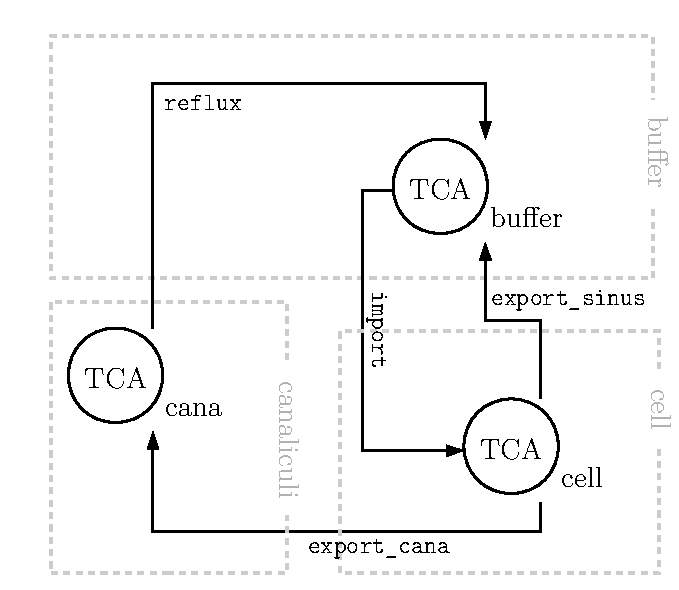
\includegraphics[width = \textwidth]{images/flowchart}
	\end{minipage}
	\caption{Differential equations and flowchart of the reaction network. Taurocholic acid,  TCA, is transported between three compartments by four different processes. (A) Assuming mass-action kinetics, the three dynamic states satisfy a set of coupled differential equations. (B) The equations are visualized in a flowchart. }
	\label{fig:flowchart}
\end{figure}

\subsection{Simulation and prediction}

Each transportation process is modeled by mass-action kinetics. The implementation in \pkg{dMod} would be as follows:
\begin{CodeChunk}
	\begin{CodeInput}
# Add reactions
reactions <- NULL
reactions <- addReaction(reactions, "TCA_buffer", "TCA_cell",
			 rate = "import*TCA_buffer",
			 description = "Uptake")
reactions <- addReaction(reactions, "TCA_cell", "TCA_buffer",
			 rate = "export_sinus*TCA_cell",
			 description = "Sinusoidal export")
reactions <- addReaction(reactions, "TCA_cell", "TCA_cana",
			 rate = "export_cana*TCA_cell",
			 description = "Canalicular export")
reactions <- addReaction(reactions, "TCA_cana", "TCA_buffer",
			 rate = "reflux*TCA_cana",
			 description = "Reflux into the buffer")

# Translate into ODE model
mymodel <- odemodel(reactions, modelname = "bamodel")

# Generate prediction function from ODE model
x <- Xs(mymodel, condition = NULL)
	\end{CodeInput}
\end{CodeChunk}
The reactions are collected in an \code{eqnlist} object. The \code{odemodel()} command composes the single reactions to an ODE system and auto-generates the \proglang{C} code which is used by the \pkg{deSolve} package to evaluate the ODE. Prediction functions generated by the \code{Xs()} command are wrapper functions for the call of \code{ode()}. The "s" in \code{Xs()} refers to "sensitivities", i.e the prediction function not only computes and returns the model prediction but sensitivities, too. The usage of the prediction function is illustrated by the following code chunk. Time points are defined between 0 and 50, numeric values are assigned to all model parameters. Finally the prediction function is called and the result, a prediction list, is plotted, shown in Figure~\ref{fig:prediction}A.

\begin{CodeChunk}
\begin{CodeInput}
times <- seq(0, 50, .1)
pars <- c(TCA_buffer = 1,
          TCA_cell = 0,
	  TCA_cana = 0,
	  import = 0.2,
	  export_sinus = 0.2,
	  export_cana = 0.04,
	  reflux = 0.1)

# Generate the prediction
out <- x(times, pars)
plot(out)

# Get sensitivities for the dynamic parameters
out <- getDerivs(x(times, pars[4:7], fixed = pars[-(4:7)]))
plot(out)
\end{CodeInput}
\end{CodeChunk}

\begin{figure}[ht]
	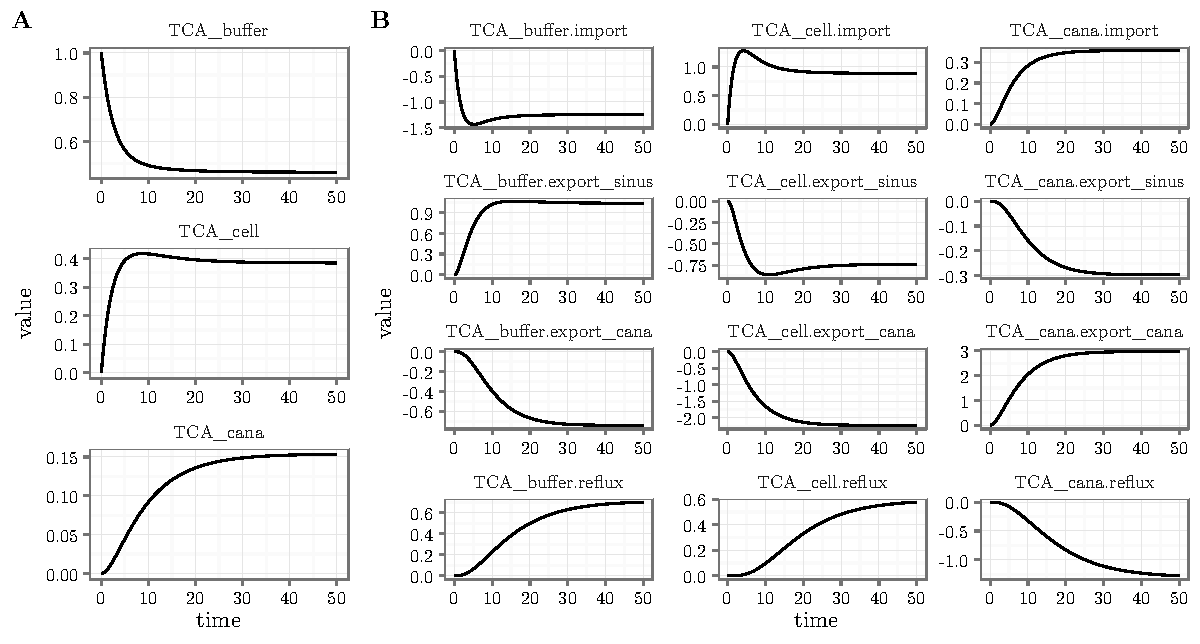
\includegraphics[width = \textwidth]{images/figure1}
	\caption{Output of the prediction function. (A) Prediction of the TCA states. (B) Sensitivities of the three TCA states with respect to the rate parameters.}
	\label{fig:prediction}
\end{figure}

Figure~\ref{fig:prediction}A shows the uptake of TCA in the cell and canaliculi, saturating around $t = 50$. The prediction parametrically depends on initial values and rate parameters. Figure~\ref{fig:prediction}B shows the model sensitivities $\frac{\partial x}{\partial p}$ for the rate parameters.

\subsection{Observation function and simulated data}
The three dynamic states, \code{TCA_buffer}, \code{TCA_cell} and \code{TCA_cana} cannot be directly measured. In practice, the cellular fraction, i.e. both cells and canaliculi, can be separated from the buffer. The radioactivity in the two fractions is determined independently. In summary, we find the following relation between the radioactive counts and the dynamic states of our ODE model:
\begin{equation}
	\begin{aligned}
		\verb!buffer! &= \verb!s * TCA_buffer!\\
		\verb!cellular! &= \verb!s * (TCA_cana + TCA_cell)!
	\end{aligned}
	\label{}
\end{equation}
The scaling factor \code{s} translates amounts into radioactive counts. The fact that the cellular fraction contains cells as well as canaliculi is represented by the sum. The implementation in \pkg{dMod} follows.

First, observables are defined by an \code{eqnvec} object from which an observation function \code{g} is generated by the \code{Y()} command. The \code{Y()} command needs to be informed which of the symbols are variables (dynamic states) or parameters. For convenience, this can be done passing the \code{reactions} that underly our ODE model.
\begin{CodeChunk}
\begin{CodeInput}
# Generate observation function
observables <- eqnvec(
  buffer = "s*TCA_buffer",
  cellular = "s*(TCA_cana + TCA_cell)"
)

g <- Y(observables, reactions, condition = NULL,
       compile = TRUE, modelname = "obsfn")

\end{CodeInput}
\end{CodeChunk}
The data we are going to simulate is for an efflux experiment, i.e. time point $t = 0$ reflects the distribution of TCA after uptake. Hence, we reset some of the parameter values. Initial values are set to steady state values. The incubation buffer is replaced by fresh buffer, meaning that \code{TCA_buffer} is set to 0. Finally, we assume that \code{s = 1000}. The prediction of the observables is made by concatenation of \code{g} and \code{x} via the concatenation operator \code{"*"} being defined in \pkg{dMod} for prediction, observation and parameter functions.
\begin{CodeChunk}
\begin{CodeInput}
# Reset parameter values
pars["TCA_cell"] <- 0.3846154
pars["TCA_cana"] <- 0.1538462
pars["TCA_buffer"] <- 0
pars["s"] <- 1e3

out <- (g*x)(times, pars, conditions = "standard")
\end{CodeInput}
\end{CodeChunk}
Finally, we obtain the simulated data by taking a subset of the prediction. At this point we make use of the "conditions" argument which allows to request a prediction for a vector of conditions, if provided by the prediction function\footnote{Both, \code{x} and \code{g} have been initialized with \code{condition = NULL} which means they are generic prediction functions and yield the same prediction for any of the requested conditions. The concept is further illustrated in Section~\ref{sec:conditions}.}. Data uncertainties $\sigma$ are derived by the Poisson nature of radioactive count experiments, i.e. $\sigma_x = \sqrt{x}$. To avoid division by 0, the minimal $\sigma$-value is set to 1. Random values are added to the predicted values to simulate observation noise. In the end, the \code{data.frame} is converted into a \code{datalist} object.
\begin{CodeChunk}
\begin{CodeInput}
# Simuate data
timesD <- c(0.1, 1, 3, 7, 11, 15, 20, 41)
datasheet <- subset(wide2long(out),
                    time %in% timesD & name %in% names(observables))
datasheet$sigma <- sqrt(datasheet$value + 1)
datasheet$value <- rnorm(nrow(datasheet), datasheet$value, datasheet$sigma)

data <- as.datalist(datasheet)

plot(out, data)
\end{CodeInput}
\end{CodeChunk}
Both, the simulated data and the model prediction from which the data is derived are shown in Figure~\ref{fig:observation}.
\begin{figure}[ht]
	\centering
	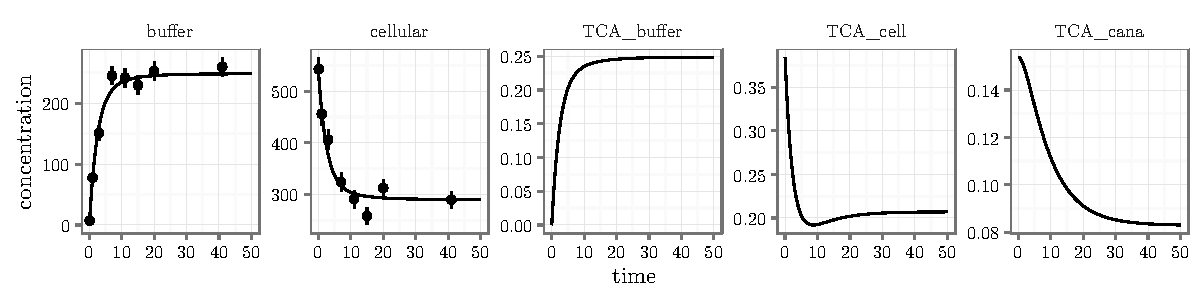
\includegraphics[width = \textwidth]{images/figure2}
	\caption{Model prediction of the internal states and observables. Simulated data is shown as dots with error bars.}
	\label{fig:observation}
\end{figure}

\subsection{Parameter transformation}
Parameter transformations play a crucial role in the set-up of \pkg{dMod}. They can have several purposes such as fixing paramer values, implementing parameter bounds, including steady-state constraints or mapping parameters to different conditions.

First, we use parameter transformations to constrain all parameters to be positive or zero because all our parameters are either amounts or rate parameters. The parameter transformation is generated by the \code{P()} command from an \code{eqnvec} object, explicitly stating the relation between the \textbf{inner} parameters, i.e.~the parameter values that are evaluated within the model, and the \textbf{outer} parameters, i.e.~the parameter values handed by the user or by an optimizer, from which the inner parameters are computed. The corresponding code reads:
\begin{CodeChunk}
\begin{CodeInput}
p <- P(
  trafo = eqnvec(
    TCA_buffer = "0",
    TCA_cell = "exp(TCA_cell)",
    TCA_cana = "exp(TCA_cana)",
    import = "exp(import)",
    export_sinus = "exp(export_sinus)",
    export_cana = "exp(export_cana)",
    reflux = "exp(reflux)",
    s = "exp(s)"
  ),
  condition = "standard"
)

outerpars <- getParameters(p)
pouter <- structure(rep(-1, length(outerpars)), names = outerpars)
plot((g*x*p)(times, pouter), data)
\end{CodeInput}
\end{CodeChunk}
The vector \code{outerpars} is the collection of all symbols on the right-hand side of \code{trafo}. It agrees with \code{names(pars)} except for \code{TCA_buffer}, which is fixed to 0 by the transformation. However, the meaning of the parameters has changed since now their values are on a log-scale. All three functions, the observation function, prediction function and parameter transformation can be concatenated to one new prediction function, \code{g*x*p} which takes times and values of the outer parameters to predict internal and observable states. The model prediction generated by \code{pouter} is shown in Figure~\ref{fig:gxp}.
\begin{figure}[ht]
	\centering
	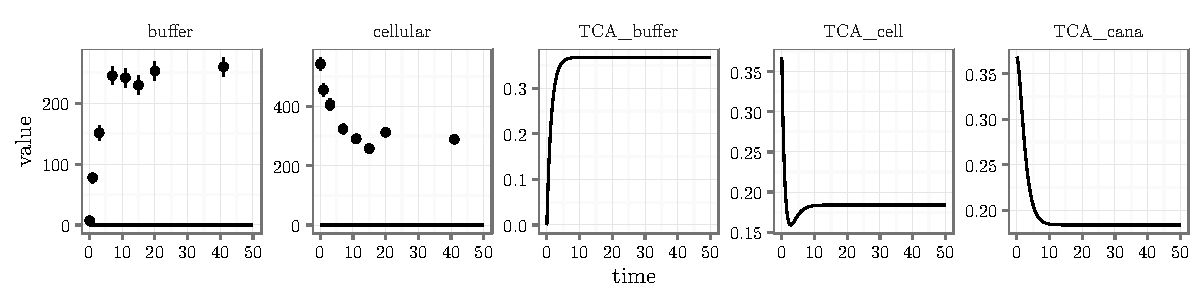
\includegraphics[width = \textwidth]{images/figure3}
	\caption{Prediction of internal and observed states. All values of the outer parameters have been set to $-1$. Simulated data points are shown as dots with error bars.}
	\label{fig:gxp}
\end{figure}

\subsection{Objective function and model fitting}
For nomally distributed measurement noise, maximum-likelihood estimation is equivalent to least-squares estimation. A least-squares objective function can be generated by the \code{normL2()} command which requires a \code{datalist} object, in our case \code{data}, and a prediction function, in our case \code{g*x*p}.

Frequently, non-identifiable parameters are encountered in non-linear dynamic systems. To prevent the optimizer from taking extreme parameter values for which the ODE solver crashes, a general $L_2$ prior can be used on all parameters, being implemented by the \code{constraintL2()} command. The command returns an \code{objfn} objection, as does \code{normL2()}. Both can be added by the \code{"+"} operator.

The following code illustrates the implementation of the objective function and how it is used with the \code{trust()} optimizer from the \pkg{trust} package to obtain a model fit, shown in Figure~\ref{fig:myfit}.

\begin{CodeChunk}
\begin{CodeInput}
obj <- normL2(data, g*x*p) + constraintL2(pouter, sigma = 10)
myfit <- trust(obj, pouter, rinit = 1, rmax = 10)

plot((g*x*p)(times, myfit$argument), data)
\end{CodeInput}
\end{CodeChunk}


\begin{figure}[ht]
	\centering
	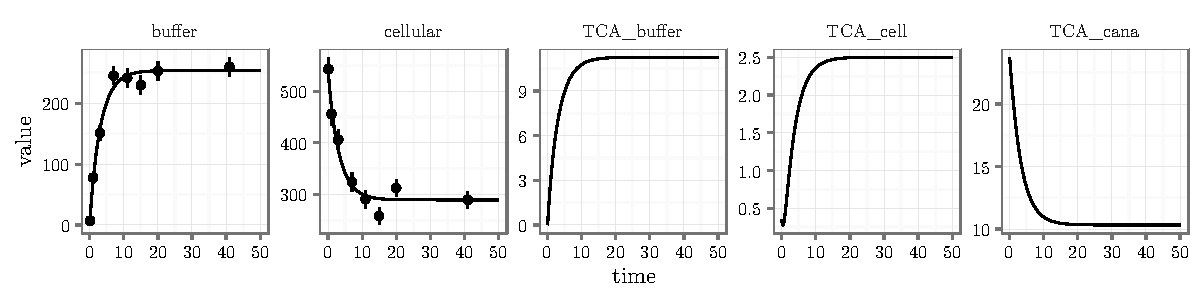
\includegraphics[width = \textwidth]{images/figure4}
	\caption{Prediction of internal and observed states after optimization of the objective function. Simulated data points are shown as dots with error bars.}
	\label{fig:myfit}
\end{figure}

Besides non-identifiability of parameters, local optima is another feature of non-linear optimization. The \code{trust()} optimizer employs derivative information and therefore, if starting within a certain radius around a local optimum, is very efficient in finding it back. Once an optimum is found, we can be confident that there is no deeper point around. However, to be confident that an optimum is the globally best solution, we might want to scatter starting points for optimization runs all over the parameter space. The \pkg{dMod} package provides the \code{mstrust()} function based on \code{trust()} to do a multi-start search:
\begin{CodeChunk}
\begin{CodeInput}
out_mstrust <- mstrust(obj, pouter, rinit = 1, rmax = 10, iterlim = 500,
                       sd = 4,
                       cores = 4, fits = 50)

myframe <- as.parframe(out_mstrust)

plotValues(myframe, value < 100)
plotPars(myframe, value < 100)
\end{CodeInput}
\end{CodeChunk}
Here, we have searched according to $\vec p_i = \vec p_0 + \Delta\vec p_i$ where $\vec p_0$ is the center, in our case \code{pouter}, $\Delta\vec p_i\sim N(0, \sigma^2)$ is a random parameter vector taken from a normal distribution, in our case $\sigma = 4$, and the index $i$ runs from 1 to \code{fits = 50}. The \code{mclapply()} command from the \pkg{parallel} package is used internally to run fits in parallel, here \code{cores = 4}. The result of \code{mstrust()} is a list of all returned values of \code{trust()}. To extract the final objective value, parameter values, convergence information and the number of interations, \code{as.parframe()} is used. The multi-start approach identifies four local optima, see Figure~\ref{fig:mstrust}, which yield almost the same objective value, Figure~\ref{fig:mstrust}A.
\begin{figure}[ht]
	\centering
	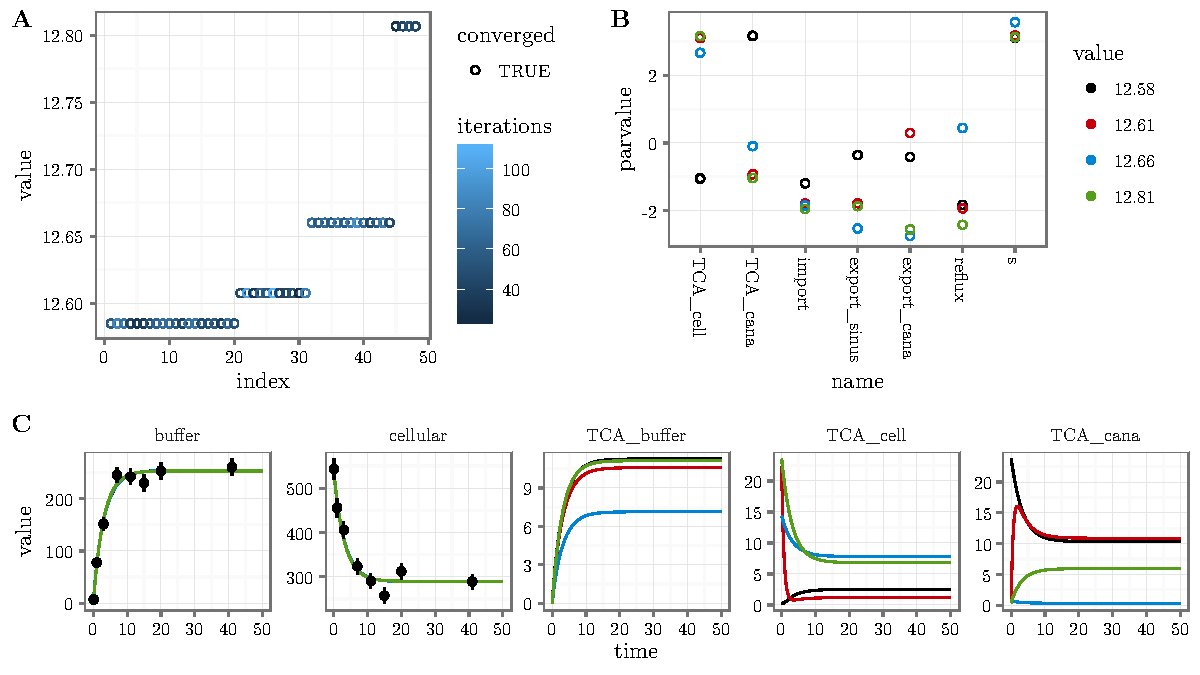
\includegraphics[width = \textwidth]{images/figure5}
	\caption{Result of multi-start fitting procedure. (A) Fits have been sorted by increasing least squares value. Four optima were found with almost identical objective value. (B) The parameter values for different optima are shown in different colors }
	\label{fig:mstrust}
\end{figure}
Despite the similar objective value, the optima are not close to each other in parameter space, as being illustrated by Figure~\ref{fig:mstrust}B. From the initial value parameters \code{TCA_cell} and \code{TCA_cana} it seems that they are exchangeable. Where \code{TCA_cell} is high, \code{TCA_cana} is low and vice versa. This is not surprising because the observed cellular TCA amount is the sum of both. A new experiment needs to be designed to distinguish one situation from another.

\subsection{Working with several conditions}\label{sec:conditions}

In practice, the canaliculi only form a closed compartment if Ca$^{2+}$/Mg$^{2+}$ ions are present in the buffer. Therefore, if the experiment is repeated with Ca$^{2+}$/Mg$^{2+}$-free efflux buffer, the contents of the canaliculi escapes quickly into the buffer compartment and the observables \code{buffer} and \code{cellular} effectively reflect \code{TCA_buffer + TCA_cana} and \code{TCA_cell}. Mathematically, two experimental conditions which differ only by the \code{reflux} parameter need to be combined in one objective function.

Like before, we generate a simulated data set. Then, a parameter transformation for the additional condition is set up and the parameter space is explored by a multi-start fit.

\begin{CodeChunk}
\begin{CodeInput}
pars["reflux"] <- 1e3
out <- (g*x)(times, pars, conditions = "open")

datasheet <- subset(wide2long(out),
		    time %in% timesD & name %in% names(observables))
datasheet$sigma <- sqrt(datasheet$value + 1)
datasheet$value <- rnorm(nrow(datasheet), datasheet$value, datasheet$sigma)

data <- data + as.datalist(datasheet)
\end{CodeInput}
\end{CodeChunk}
Similar to objective functions and observation/prediction/parameter functions, as we will see, datalists can be combined by the \code{"+"} operator.

To add a condition to the parameter transformation function, we use the equations of the standard condition as a template for the "open" condition. Parameter transformation functions for different conditions are combined by the \code{"+"} operator.

\begin{CodeChunk}
\begin{CodeInput}
trafo <- summary(p)$standard$equations
trafo["reflux"] <- "exp(reflux_open)"
p <- p + P(trafo, condition = "open")
\end{CodeInput}
\end{CodeChunk}

Compared to the situation before we have gained the outer parameter \code{reflux_open}. Both transformations, "standard" and "open", evaluate the same vector of outer parameters meaning that they yield the same values for all but \code{reflux} and \code{reflux_open}. The prediction function \code{g*x} is generic in the sense that \code{condition = NULL} whereas the concatenation \code{g*x*p} has the conditions "standard" and "open", evaluating the identical function \code{g*x} on two parameter vectors.

We define an updated objective function:
\begin{CodeChunk}
\begin{CodeInput}
outerpars <- getParameters(p)
pouter <- structure(rep(-1, length(outerpars)), names = outerpars)

obj <- normL2(data, g*x*p) + constraintL2(pouter, sigma = 10)
\end{CodeInput}
\end{CodeChunk}

Then we start 50 fits around \code{pouter}. The list of fits is simplified to a \code{parframe} and by the \code{as.parvec()} function, the parameter vector (of the best fit) is extracted from the \code{parframe}. The best fit is used to make a prediction and plot it together with the simulated data. All results are shown in Figure~\ref{fig:twoconditions}.

\begin{CodeChunk}
\begin{CodeInput}
out_mstrust <- mstrust(obj, pouter, rinit = 1, rmax = 10, iterlim = 500,
		       sd = 4,
		       cores = 4, fits = 50)
myframe <- as.parframe(out_mstrust)
plotValues(myframe, value < 100)
plotPars(myframe, value < 100)

bestfit <- as.parvec(myframe)
plot((g*x*p)(times, bestfit), data)
\end{CodeInput}
\end{CodeChunk}
\begin{figure}[ht]
	\centering
	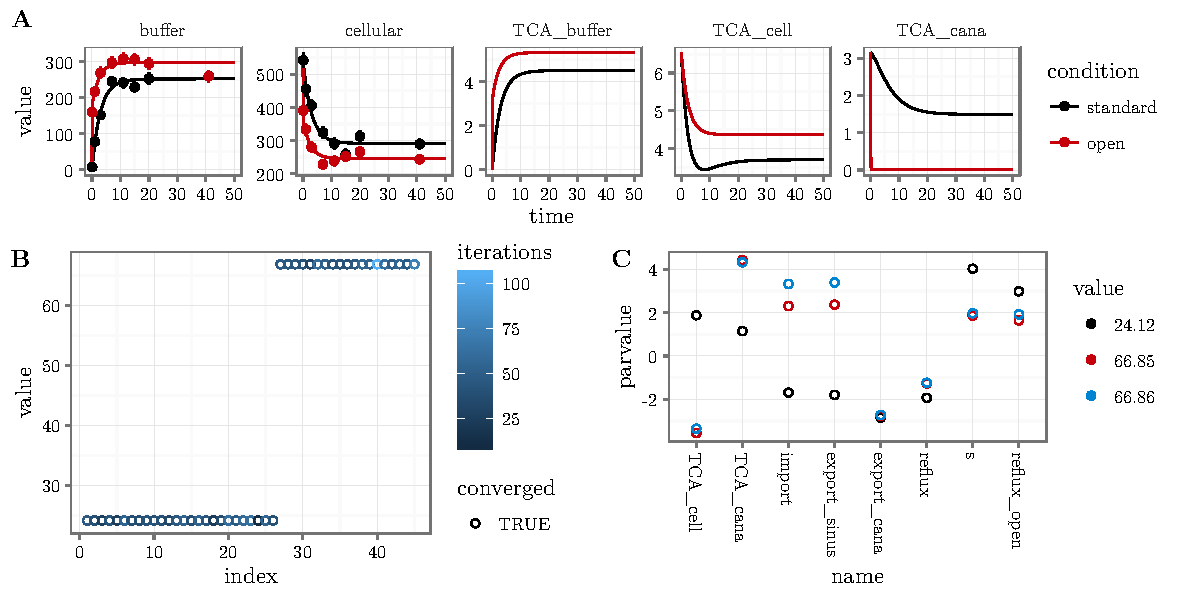
\includegraphics[width = \textwidth]{images/figure6}
	\caption{Result of multi-start fitting procedure with two experimental conditions. (A) Model prediction of the best fit and the simulated data are shown in different colors. (B) Fits have been sorted by increasing least squares value. The lowest value clearly separates from the second plateau. (C) Plotting the parameter values for each of the fits reveals that the second plateau consists of two optima. The lowest plateau however corresponds to a unique optimum.}
	\label{fig:twoconditions}
\end{figure}

Interestingly, with the new experiment the best optimum becomes unique. The log-likelihood difference, i.e.~half the difference between the objective values, is more than 20 between the lowest and the second plateau, which is highly significant. The uniqueness of the lowest plateau is confirmed by Figure~\ref{fig:twoconditions}C which shows no scattering of the black circles.

\subsection{Parameter uncertainty and identifiability}

One might wonder why the optimum is unique as for any choice of the scaling parameter \code{s} we find appropriate values of the TCA initial value parameters that give rise to exactly the same prediction of the observables. The reason for the uniqueness is the parameter $L_2$-constraint that we have added to the objective function. Nonetheless, we will see, that the non-identifiability is still visible in the profile likelihood.

The profile likelihood is computed by the \code{profile()} command. There are several options to control the step-size and accuracy. For convenience the \code{method} option can be used to select between the presets \code{"integrate"} and \code{"optimize"}.

The code
\begin{CodeChunk}
\begin{CodeInput}
profiles <- profile(obj, bestfit, names(bestfit), limits = c(-5, 5), cores = 4)
plotProfile(profiles)
plotPaths(profiles, whichPar = "s")
\end{CodeInput}
\end{CodeChunk}
gives us the result shown in Figure~\ref{fig:pl}.
\begin{figure}[ht]
	\centering
	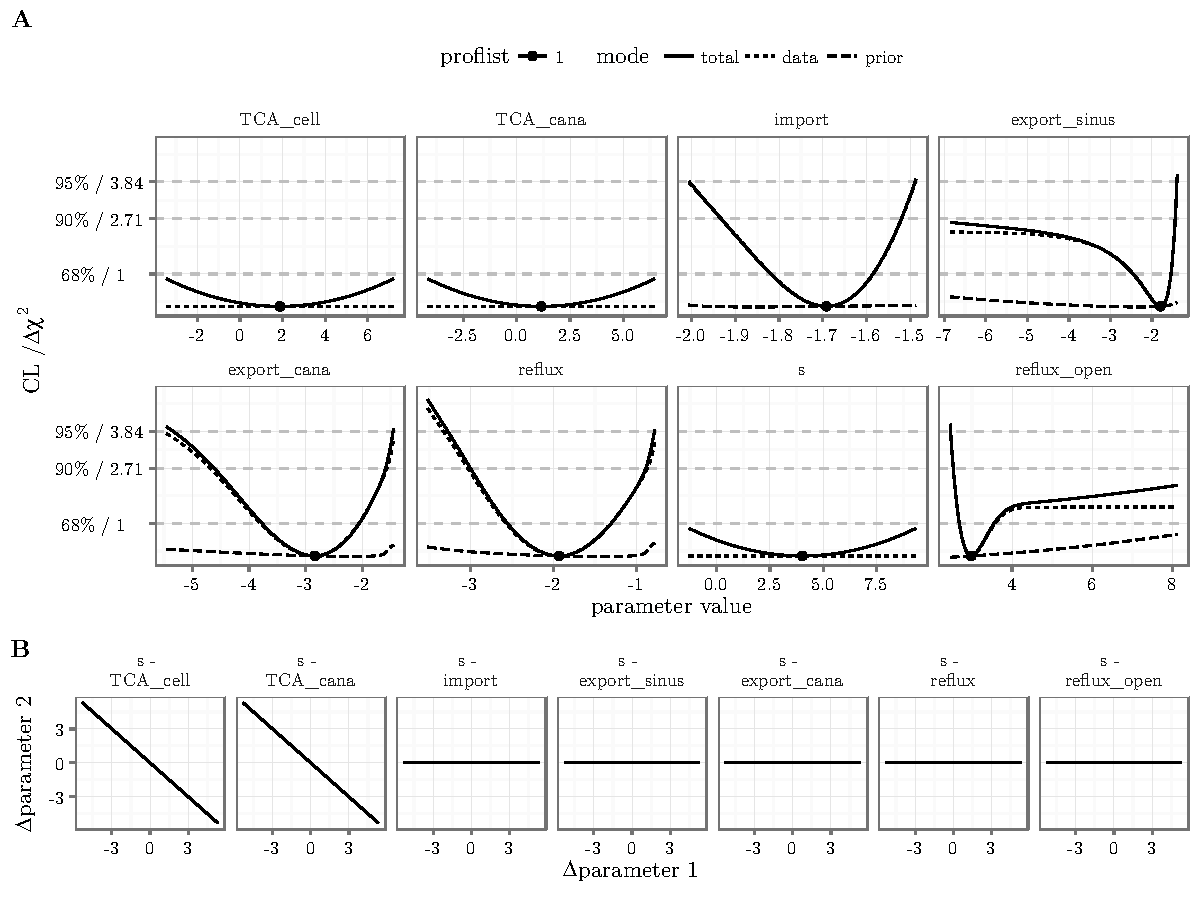
\includegraphics[width = \textwidth]{images/figure7}
	\caption{Profile likelihood. (A) Profiles of all parameters. Data- and prior contribution to the total objective value are distinguished by line-type. (B) Parameter paths for the scaling parameter \code{s}.}
	\label{fig:pl}
\end{figure}
Computing the profile likelihood, the sum of data contribution, \code{normL2}, and prior contribution, \code{constraintL2}, are optimized under the constraint of a given parameter value for the profiled parameter. In the optimum, data and prior contribution are evaluated separately giving rise to the dashed and dotted lines in Figure~\ref{fig:pl}A. As we had expected, the data contribution to the initial value parameters \code{TCA_cell}, \code{TCA_cana} and the scaling parameter \code{s} is constantly zero. The parameters are structurally non-identifiable.

Each profile corresponds to a certain path in parameter space. The path for the profile of the non-identifiable scaling parameter \code{s} is shown in Figure~\ref{fig:pl}B. It shows a clear coupling of scaling and the initial value parameters: both initial value parameters have to be decreased by the same extent as the scaling parameter is increased to keep the prediction unchanged.

The parameters \code{export_sinus} and \code{reflux_open} exceed the 95\% confidence threshold only to one side. Given the data, the \code{export_sinus} parameter could equally be $-\infty$ (corresponding to an export rate of 0) without changing the likelihood significantly to the worse. A similar statement holds for the \code{reflux_open} parameter which could equally be $\infty$ meaning that we could assume instantaneous draining of the canaliculi for the \code{"open"} condition. The two parameters are practically non-identifiable and allow to reduce the model.

Finally, the parameters \code{import}, \code{export_cana} and \code{reflux} exceed the 95\% confidence threshold in both directions meaning that the parameters have finite confidence intervals. However, the confidence intervals are rather large and we might ask if there is further information that we could use to improve parameter identifiability without generating new data.

\subsection{Steady-state constraints and implicit transformations}

So far we have estimated both initial concentrations, \code{TCA_cell} and \code{TCA_cana}, independently. However, we know that the efflux experiment was just started after completion of the uptake process. Our system runs into a steady state, the buffer is exchanged and the measurement begins. Hence, we can use the steady-state condition as an additional information for the modeling process.

The steady-state relation between \code{TCA_cana} and \code{TCA_cell} can be derived analytically from the ODE, Figure~\ref{fig:flowchart}A. It reads
\begin{equation}
	\verb!TCA_cana! = \verb!export_cana * TCA_cell / reflux!
	\label{}
\end{equation}
This relation can be explicitly used in a parameter transformation to express \code{TCA_cana} in terms of other parameters. The dimension of the parameter space is thereby reduced by one. The following implementation shows how we would use the existing transformation function \code{p} to generate an alternative transformation function \code{pSS} to replace \code{p} in the prediction function \code{g*x*p}.
\begin{CodeChunk}
\begin{CodeInput}
pSS <- NULL
trafos <- summary(p)
conditions <- names(trafos)
for (n in conditions) {

  equations <- trafos[[n]]$equations
  equations["TCA_cana"] <- "exp(export_cana)*exp(TCA_cell)/exp(reflux)"
  pSS <- pSS + P(equations, condition = n)
  
}
\end{CodeInput}
\end{CodeChunk}
We get all the information about the transformations from the \code{summary()} command. The equation for \code{TCA_cana} is substituted by our steady-state constraint. By the \code{"+"} operator, a new parameter transformation function \code{pSS} for our multiple conditions is constructed step-by-step.

Next, we want to implement the steady-state constraint by an implicit parameter transformation. Let $\dot x = f(x, p)$ be our dynamic system. Then, under certain conditions, we find a function $g(p)$ such that $f\big( g(p), p\big) = 0$ for all $p$ i.e.~$x_S = g(p)$ is a steady state of $f$. The parameter transformation we want to generate is the function $p \mapsto \big(p, g(p)\big)$. Here, the set of outer parameters is the set of the reaction rates  $p$ whereas the set of inner parameters contains these rates and the corresponding steady states as initial value parameters. The root of $f$ must be determined numerically which is implemented based on \code{multiroot()} from the \pkg{rootSolve} package.

The following code is a reimplementation of the example above. The condition "open" is special in that the reflux rate is modified compared to the reflux rate by which the steady state is computed. This is solved by an event, flipping a switch variable from 0 to 1 and thereby replacing the rate \code{reflux} by \code{reflux_open}. 

\begin{CodeChunk}
\begin{CodeInput}
# Add reactions
reactions <- NULL
reactions <- addReaction(reactions, "TCA_buffer", "TCA_cell",
		 rate = "import*TCA_buffer",
		 description = "Uptake")
reactions <- addReaction(reactions, "TCA_cell", "TCA_buffer",
		 rate = "export_sinus*TCA_cell",
		 description = "Sinusoidal export")
reactions <- addReaction(reactions, "TCA_cell", "TCA_cana",
		 rate = "export_cana*TCA_cell",
		 description = "Canalicular export")
reactions <- addReaction(reactions, "TCA_cana", "TCA_buffer",
		 rate = "(reflux*(1-switch) + reflux_open*switch)*TCA_cana",
		 description = "Reflux into the buffer")
reactions <- addReaction(reactions, "0", "switch",
		 rate = "0",
		 description = "Create a switch")

# Translate into ODE model
mymodel <- odemodel(reactions, modelname = "bamodel")
\end{CodeInput}
\end{CodeChunk}

For the implicit parameter transformation we need the ODE which is obtained by the \code{as.eqnvec()} command from the reactions, an \code{eqnlist} object. The Jacobian of $f$ is rank-deficient because the system has a conserved quantity $c$, i.e.~\code{TCA_tot = TCA_buffer + TCA_cana + TCA_cell}. Replacing one element of $f$ by $c - \verb!TCA_tot!$, the rank of the Jacobian is completed, the condition for the local existence of the implicit function $g(p)$ is satisfied and the steady state is parameterized by $p$ and the additional parameter \code{TCA_tot}.

\begin{CodeChunk}
\begin{CodeInput}
# Set up implicit parameter transformation
f <- as.eqnvec(reactions)[c("TCA_buffer", "TCA_cana", "TCA_cell")]
f["TCA_cell"] <- "TCA_buffer + TCA_cana + TCA_cell - TCA_tot"
pSS <- P(f, "TCA_tot", method = "implicit",
         compile = TRUE, modelname = "pfn")
\end{CodeInput}
\end{CodeChunk}

For the optimization, all outer parameters should still be log-parameters, an explicit parameter transformation. The final transformation will be a concatenation of the implicit and explicit transformations, \code{pSS*p}.

\begin{CodeChunk}
\begin{CodeInput}
# Set up explicit parameter transformation
innerpars <- unique(c(getParameters(mymodel),
                      getSymbols(observables),
                      getSymbols(f)))
trafo <- as.eqnvec(innerpars, names = innerpars)
trafo[reactions$states] <- "0"
trafo <- replaceSymbols(innerpars,
                        paste0("exp(", innerpars, ")"),
                        trafo)
p <- P(trafo)
\end{CodeInput}
\end{CodeChunk}

Both, the exchange of buffer and the opening of bile canaliculi by a Ca$^{2+}$/Mg$^{2+}$-free buffer are implemented as events. We therefore have different prediction functions for the two conditions.

\begin{CodeChunk}
\begin{CodeInput}
# Set up prediction function with events
event.buffer <- data.frame(var = "TCA_buffer", 
			   time = 0, 
			   value = 0, 
			   method = "replace")
event.open   <- data.frame(var = "switch", 
			   time = 0, 
			   value = 1, 
			   method = "replace")

x <- Xs(mymodel, 
	events = event.buffer, 
	condition = "standard") +
     Xs(mymodel, 
        events = rbind(event.buffer, event.open), 
	condition = "open")
\end{CodeInput}
\end{CodeChunk}

Although the observables have not changed compared to the set-up with purely explicit transformations, the observation function must be generated again because the new parameter \code{TCA_tot} has appeared. This parameter is not contained in the reactions. Therefore, we use the \code{states} and \code{parameters} arguments to explicitly inform the observation function about the states and parameters involved. Otherwise, parameter sensitivities are not propagated correctly.

\begin{CodeChunk}
\begin{CodeInput}
# Generate observation function with modified states/parameters
g <- Y(observables,
       states = reactions$states,
       parameters = setdiff(innerpars, reactions$states),
       compile = TRUE, modelname = "obsfn")
\end{CodeInput}
\end{CodeChunk}

Finally, the objective function is defined. The prediction function is now a concatenation of four functions.

\begin{CodeChunk}
\begin{CodeInput}
# Generate objective function
outerpars <- getParameters(p)
pouter <- structure(rep(-1, length(outerpars)), names = outerpars)
obj <- normL2(data, g*x*pSS*p) + constraintL2(pouter, sigma = 10)
\end{CodeInput}
\end{CodeChunk}

The same simulated data set has been fitted by the fully explicit and the implicit/explicit model implementations. In both cases the global optimum is unique. Parameter profiles have been computed with both model implementations, shown in Figure~\ref{fig:allprofiles}.
\begin{figure}[ht]
	\centering
	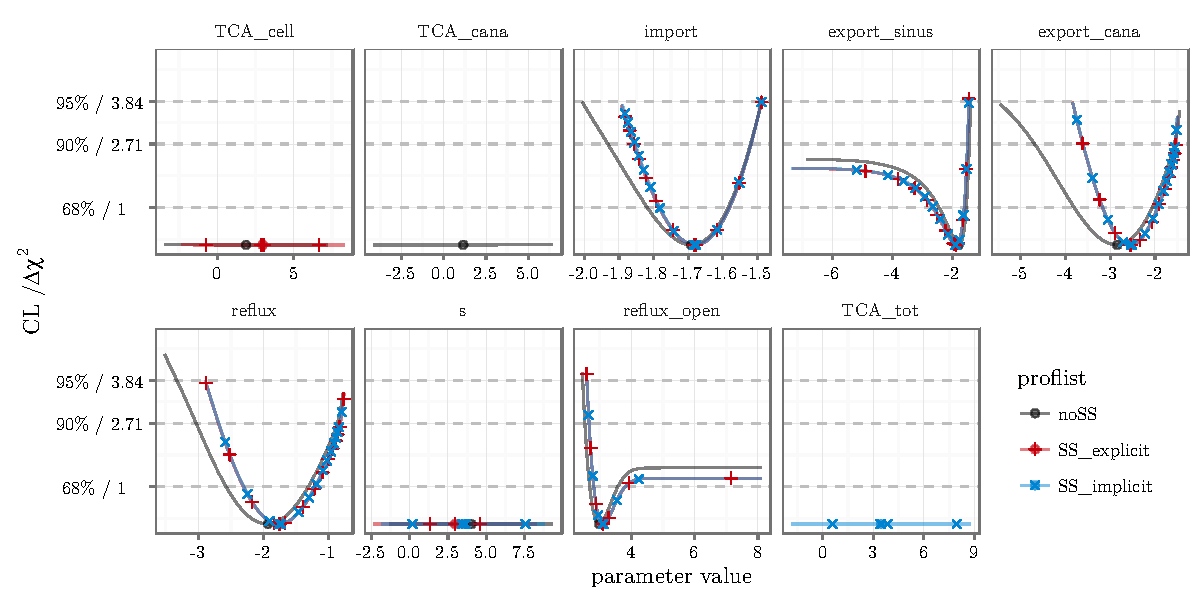
\includegraphics[width = \textwidth]{images/figure8}
	\caption{Comparison of parameter profiles. The profile likelihood for the model without steady-state constraints, explicit steady-state constraints and implicit implementation of steady states is visualized by different colors.}
	\label{fig:allprofiles}
\end{figure}
The optima found by all three approaches are statistically compatible. The two implementations using the steady-state information show exactly the same profiles. Since one formulation is parameterized by \code{TCA_cell} whereas the other is parameterized by \code{TCA_tot}, the plot highlights one of the fundamental properties of the profile likelihood: invariance under reparameterization. In comparison to the profiles without steady-state information, the new profiles are narrower, meaning that the parameters are better identifiable. This was to be expected because we have reduced the dimension of the parameter space by one.

\subsection{Prediction uncertainty and validation profiles}

Combining the steady-state constraint and two efflux experiments, one with closed canaliculi and the other with open canaliculi, we could fully identify the rate parameters \code{import}, \code{export_cana} and \code{reflux}. The amount parameter \code{TCA_tot} is fully coupled with the scaling parameter \code{s} such that both are structurally non-identifiable. The parameters \code{export_sinus} and \code{reflux_open} are practically non-identifiable since both parameters cannot be constrained to a finite interval with 95\% confidence.

Next, we investigate the possibility to predict cellular amounts of TCA, \code{TCA_cell}, despite the non-identifiability of parameters. Certainly, it is necessary to fix the scale by including the knowledge about the total TCA amount which is 1. A prediction profile is computed based on a test data point

\begin{CodeChunk}
\begin{CodeInput}
obj.validation <- datapointL2(name = "TCA_cell", 
			      time = 41, 
			      value = "d1", 
			      sigma = .002, 
			      condition = "standard")
\end{CodeInput}
\end{CodeChunk}

for the dynamic state \code{TCA_cell} at time $t = 41$ under the "standard" condition. The uncertainty $\sigma = 0.002$ is set to a small value, i.e. below 1\% of the prediction value. The \code{datapointL2()} command returns an objective function which evaluates the model prediction\footnote{Several objective function combined by the \code{"+"} operator share the same environment. Thus, the prediction computed by the first objective function can be evaluated by all other functions to come.} and computes the least-squares function of the test datapoint, returning derivatives for the data-point parameter \code{d1}.

The derivative information for \code{d1} is used by the \code{profile()} function to compute the profile likelihood with respect to this parameter:

\begin{CodeChunk}
\begin{CodeInput}
myfit <- trust(obj + obj.validation, 
	       parinit = c(d1 = 1, bestfit[-7]), 
	       fixed = c(TCA_tot = log(1)), 
	       rinit = 1, rmax = 10)

profile_prediction <- profile(obj + obj.validation, 
			      myfit$argument, "d1", limits = c(-5, 5), 
			      fixed = c(TCA_tot = log(1)))
\end{CodeInput}
\end{CodeChunk}

First, we obtain the new parameter estimate \code{myfit$argument} with the new data-point parameter \code{d1} for fixed \code{TCA_tot} amount. The \code{profile()} function must be informed about the fixed parameter, too. The result is shown in Figure~\ref{fig:validation}A.  

\begin{figure}[ht]
	\centering
	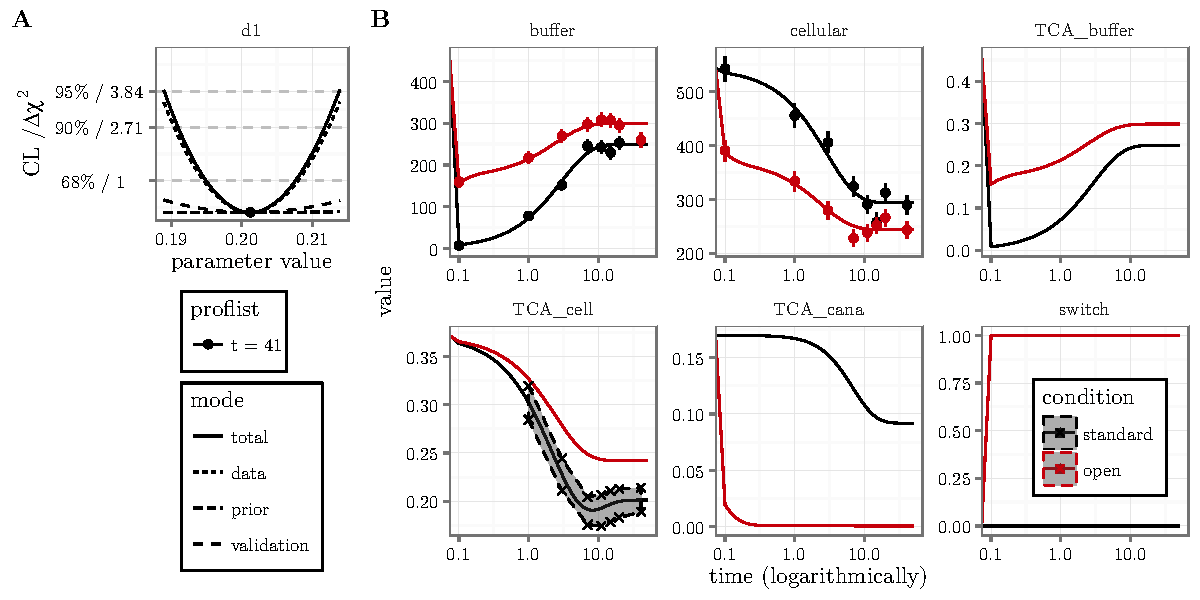
\includegraphics[width = \textwidth]{images/figure9}
	\caption{Validation profile and confidence bands for model prediction. (A) The profile likelihood for the data point parameter \code{d1} describing \code{TCA\_cell} at time point $t = 41$ was computed. (B) The same computation for different time points yields 95\% confidence bands on the prediction of \code{TCA\_cell}.}
	\label{fig:validation}
\end{figure}

Changing the data-point parameter \code{d1}, the model is quickly forced to follow the new data point. This is apparent from the "validation" contribution to the total objective value. It remains small with respect to the "data" contribution originating from all other data points. Forcing the model prediction to deviate more than $0.01$ from the original one, the profile exceeds the 95\% confidence threshold providing a confidence interval for the prediction itself. The procedure has been repeated for several time points to produce a confidence band for the cellular TCA prediction, shown in Figure~\ref{fig:validation}B. The 95\% confidence band is closed towards small and large amounts. 

In summary, we find that the prediction of cellular TCA amounts is highly precise despite the non-identifiability of the \code{export_sinus} and \code{reflux_open} parameters.

\section{Extensions of dMod}
\label{sec:extensions}

\bibliography{mybib}{}

\end{document}

